% !TEX root = ../../main.tex


\begin{algorithm}[t]
  \begin{flushleft}
  \caption{Affinities from Aggregated Central Instance Masks}
   \hspace*{\algorithmicindent} \textbf{Input:} Graph $\mathcal{G}(V,E)$; \maskname masks $\mathcal{M}_{\coord{u}}: \mathcal{N}_{K\times K} \rightarrow [0,1]$  \\
  \hspace*{\algorithmicindent} \textbf{Output:} Affinities $\bar{a}_e\in[0,1]$ with variance $\sigma^2_e$ for all edges $e\in E$\\
  \hspace*{\algorithmicindent} 
  \begin{algorithmic}[1]
  \footnotesize
  % \scriptsize
  % \small
      % \State Initial clustering: $\Pi=\{\{v_1\}, \ldots, \{v_{|V|}\}\}$
      % \State Initialize interactions between clusters with $ = w^+_e - w^-_e$
      \For{each edge $e=(\coord{u}, \coord{v})\in E$ in graph $\mathcal{G}$}
        \State Get coordinates $\coord{u}=(u_x,u_y)$ and $\coord{v}=(v_x,v_y)$ of pixels linked by edge $e$
        \State Collect all $T$ masks $\mathcal{M}_{\coord{c}_1},\ldots,\mathcal{M}_{\coord{c}_T}$ including both pixel $\coord{u}$ and pixel $\coord{v}$
        \State Init. vectors $[a_1,\ldots,a_T] = [\evidW_1,\ldots,\evidW_T] = 0$ for affinities and evidence weights
        \For{$i\in 1, \ldots,T$}
            \State Get relative coords. of $\coord{u}$ and $\coord{v}$ with respect to the central pixel $\coord{c}_i$
            \State $a_i \gets \min \big(\mathcal{M}_{\coord{c}_i}(\coord{u} - \coord{c}_i), \,\mathcal{M}_{\coord{c}_i}(\coord{v} - \coord{c}_i)\big)$ \Comment{Fuzzy-AND: both values active}
            \State $\evidW_i \gets \max \big(\mathcal{M}_{\coord{c}_i}(\coord{u} - \coord{c}_i), \,\mathcal{M}_{\coord{c}_i}(\coord{v} - \coord{c}_i)\big)$ \Comment{Fuzzy-OR: at least one value active}
        \EndFor
        \State Get weighted affinity average $\bar{a}_e= \sum_{i} a_i \evidW_i\,/\,\sum_{i}\evidW_i$ 
        \State Get weighted affinity variance $\sigma^2_e = \sum_{i} \evidW_i (a_i-\bar{a}_e)^2\,/\,\sum_{i}\evidW_i$
      \EndFor
      \State
      \Return $\bar{a}_e, \sigma^2_e$ for each $e\in E$
  \end{algorithmic}
    \label{alg:computing_affinities}
  \end{flushleft}

\end{algorithm}
\begin{figure}[t]
\centering
        % \includegraphics[width=0.4\textwidth,trim=0.25in 0.25in 0.68in 0.36in,clip]{./figures/LSIMasks/SSBM_experiments.pdf} % 0.45
        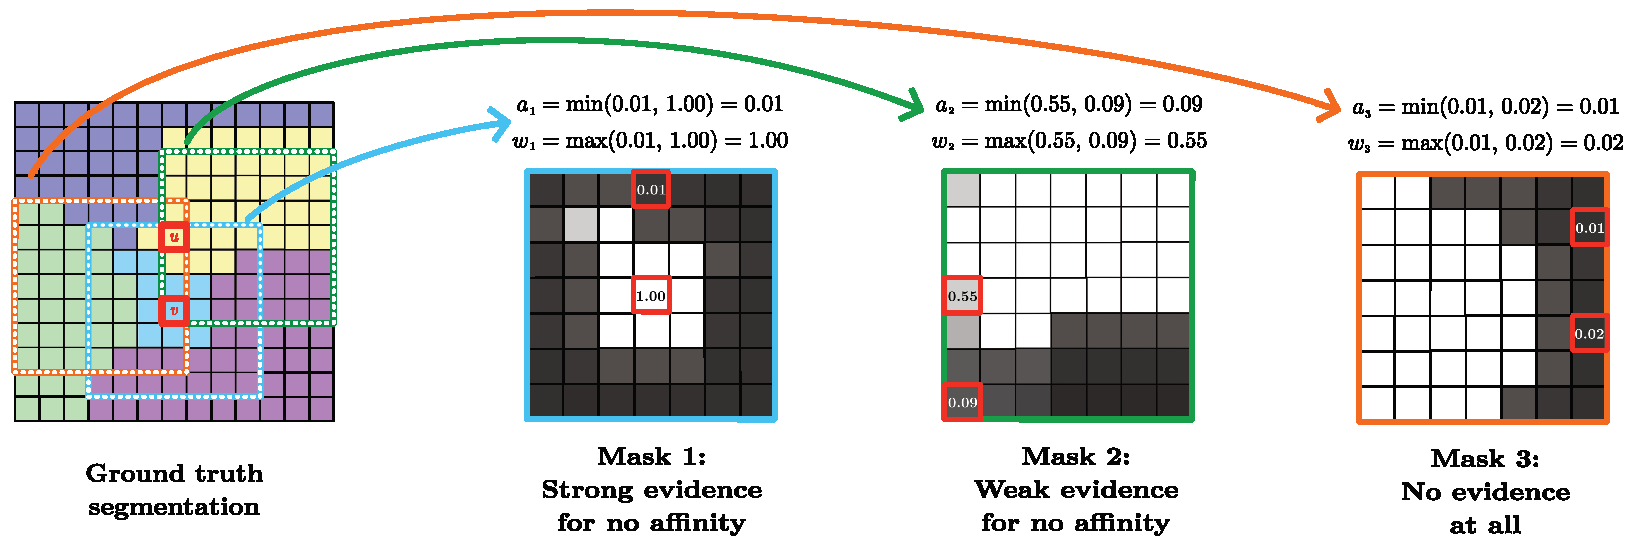
\includegraphics[width=\textwidth]{./figures/LSIMasks/mask_aggregation.pdf} % 0.45
        \caption[Proposed method to average overlapping masks]{Proposed method to average overlapping masks and compute the affinity between pixel $u$ and pixel $v$ (highlighted in red in the ground-truth segmentation on the left). For simplicity, we only consider three masks among all the ones including both pixels $u$ and $v$. 
        % For each of the three masks in the lower part of the figure, we highlight in red the predicted probabilities for $u$ and $v$ to be part of the instance that covers the central pixel of the mask. 
        In \emph{Mask 1}, only $v$ is part of the mask, so there is a strong evidence for no affinity between $u$ and $v$; in \emph{Mask 2},  $u$ is predicted to be part of the mask only with a low confidence, so the contribution of this mask in the final average will be weak; in \emph{Mask 3}, both pixels are not part of the \maskname mask, so there is no evidence about their affinity. 
        The final affinity value of edge $(u,v)$ is given by the weighted average of the collected affinities $a_i$ weighted with the evidence weights $\evidW_i$: $\bar{a}_e= \sum_{i=1}^3 a_i \evidW_i\,/\,\sum_{i}\evidW_i$
        }
    \label{fig:alg_explained}
\end{figure}


% \section{Extracting Affinities from Central Instance Masks}
\section{Affinities with Uncertainty from Aggregated Masks}\label{sec:aggr_affs}
In order to obtain an instance segmentation from the predictions of the model presented in Sec. \ref{sec:model}, we now compute instance-aware pixel-pair affinities for a given sparse $N$-neighborhood structure (see Table \ref{tab:neighborhood_structures} in supplementary material for details about the structure) and use them as edge weights of a pixel grid-graph $\mathcal{G}(V,E)$, such that each node represents a pixel / voxel of the image. The graph is then partitioned to obtain object instances.
% \TODO{Section intro} Second contribution; two ways
% In this section, we propose two ways to perform something similar and use the predicted per-pixel \maskname masks to define the edge weights of a grid-graph.

In this section, we propose an algorithm that, without the need of any threshold parameter, aggregates predictions from overlapping \maskname masks and outputs edge weights with associated uncertainty.
Related work either thresholds the predicted \maskname masks \cite{januszewski2018high,hirsch2020patchperpix,meirovitch2016multi} or computes Intersection over Union (IoU) scores for overlapping patches \cite{liu2016multi}. However, an advantage of predicting pixel-pair affinities / pseudo-probabilities as compared to IoU scores is that affinities can easily be translated into attractive and repulsive interactions in the grid-graph 
% i.e. edge with either positive or negative weights, 
and a parameter-free partitioning algorithm can be employed to yield instances.
% Related work in \cite{liu2016multi} aggregate \maskname masks by computing Intersection over Union (IoU) scores for overlapping patches, however these scores cannot be translated into attractive and repulsive cues of the graph, so hierarchical agglomerative clusterings 

Here, we propose a simple algorithm to aggregate predictions from multiple patches: Fig. \ref{fig:alg_explained} shows a simplified example of how Algorithm \ref{alg:computing_affinities} computes the affinity for an edge $e$ linking a pair of pixels $\coord{u}$ and $\coord{v}$.
As a first step, the algorithm loops over all predicted \maskname masks including both $\coord{u}$ and $\coord{v}$. 
% For example, if $\coord{u}$ and $\coord{v}$ are direct neighbors and the predicted masks have shape $K\times K$, then there will be $K(K-1)$ masks including both pixel $\coord{u}$ and $\coord{v}.$\footnote{Note that here we ignore possible boundary effects by considering two pixels close to the image border.} 
However, not all these masks are informative, as we visually explain in Fig.~\ref{fig:mask_cases}: a mask $\mathcal{M}_{\coord{c}_i}$ centered at pixel $\coord{c}_i$ provides any evidence about the affinity between pixels $\coord{u}$ and $\coord{v}$ only if at least one of the two pixels belongs to the mask (fuzzy OR operator at line 8 in Alg. \ref{alg:computing_affinities}).
If both pixels do not belong to it, we cannot say anything about whether they belong to the same instance (see Fig. \ref{fig:mask_cases}c). We model this with an evidence weight $\evidW_i\in[0,1]$, which is low when both pixels do not belong to the mask.
% If both pixels do not belong to it, then the evidence weight  goes to zero (see Fig. \ref{fig:mask_cases}c).
On the other hand, when at least one of the two pixels belongs to the mask, we distinguish two cases (fuzzy AND operator at line 7 in Alg. \ref{alg:computing_affinities}): i)
both pixels belong to the mask  (case in Fig. \ref{fig:mask_cases}a), so by transitivity we conclude they should be in the same instance and their affinity $a_i$ should tend to one; 
ii) only one pixel belongs to the mask (case in Fig. \ref{fig:mask_cases}b), so that according to this mask they are in different instances and their affinity should tend to zero. 

At the end, we compute a weighted average $\bar{a}_e$ and variance $\sigma^2_e$ of the collected affinities from all overlapping masks, such that masks with more evidence will contribute more on average, and the obtained variance is a measure of how consistent were the predictions across masks. 
The algorithm was implemented on GPU using PyTorch and the variance was computed via Welford's online stable algorithm \cite{welford1962note}.





